\documentclass[00-livre-main.tex]{subfiles}
\begin{document}

\chapter{The Equation of a Line in the Plane}


Let's recall the idea of \emph{the plane} from classical geometry: the plane is like a flat sheet of drawing paper, which extends indefinitely in all directions without bound. 
It is the playground for lots of serious considerations from high school: points, lines, circles, triangles, rectangles, and various other doodles live in it. 
I say \emph{in} it rather than \emph{on} it, because all of those objects really have their existence inside the plane. 
If we were to say ``on the plane'' then one might think of them as sitting on top of the paper, where a light breeze might move them about. 
No, those things live inside the plane just as sure as you and I live inside the universe.

And while all of that is evocative and romantic, it doesn't make doing mathematics any easier. 
Our aim in this first chapter is to do some concrete mathematics: we want to figure out how to describe a single line in the plane very carefully. 
To do this, we will use tools that Ren\'{e} Descartes taught us: coordinates. 
Better yet, we will use an update of the idea and introduce \emph{vectors}. 
Our work has to rely on something, so at some points we will make use of geometry facts you learned in high school. 
But for all of the points and vectors, angles and dot products, we will go straight to the heart of a single important question:

\begin{quotation}
\textbf{\large How can we clearly describe a single line in the plane with an equation?}
\end{quotation}

\clearpage

\section*{Points, Vectors, and Vectors}


You have likely seen the idea of \emph{Cartesian coordinates} on the plane before. To be clear, let's set things down carefully. In the plane, we choose a pair of perpendicular lines which meet at a point $O$. This special point is called the \emph{origin}. Then, we choose a point $X$ on one of the lines and draw the circle centered at $O$ which passes through $X$. Note that this circle meets our two lines in two points each, four points total, one of which is the point $X$. Then, from $X$, we rotate around the circle by a quarter turn counterclockwise until we hit one of the points on the other line. This new point we will call $Y$. Are you drawing with me? Here is my picture so far.

\begin{figure}[h!]
\centering
\begin{tikzpicture}[scale=2]
\draw (-1,4/3) -- (1,-4/3);
\draw (-3/2,-9/8) -- (3/2,9/8);
\draw (0,0) circle [radius=3/4];
\draw[->] (-50:1) arc (-50:35:1);
\node [right] at (1.1,0) {rotate counterclockwise};
\node [left] at (0,0) {$O$};
\node [below] at (9/20,-3/5) {$X$};
\node [above] at (3/5,9/20) {$Y$};
\end{tikzpicture}
\end{figure}

We call the line $OX$ the \emph{$x$-axis} and the line containing $Y$ the \emph{$y$-axis}. Here comes the amazing part: we declare the circle we used to be of \emph{unit size}, and make the lines $OX$ and $OY$ into number lines! The important part is that the point $O$ should represent $0$ on both number lines, and the points $X$ and $Y$ should each represent $1$ on their lines. So, instead of marking things with $O$, $X$, and $Y$, we put down marks where $X$ and $Y$ are and label them with $1$'s, and add little arrows marked with $x$ and $y$ near the positive ``ends'' of the lines $OX$ and $OY$, respectively.

\begin{figure}[h!]
\centering
\begin{tikzpicture}[scale=1.5]
\draw[->] (-1,4/3) -- (1,-4/3);
\draw[->] (-3/2,-9/8) -- (3/2,9/8);
\draw[fill] (9/20,-3/5) circle [radius=0.03];
\draw[fill] (3/5,9/20) circle [radius=0.03];
\node [below] at (9/20,-3/5) {$1$};
\node [above] at (3/5,9/20) {$1$};
\node [right] at (1,-4/3) {\small $x$};
\node [left] at (3/2,9/8) {\small $y$};
\end{tikzpicture}
\end{figure}

Note that above I have done something a bit silly and let the picture just fall on the paper in an unusual way. 
I really mean unusual as ``not usual.'' 
The usual way arranges the lines on the paper to match our expected horizontal ($x$) and vertical ($y$) directions. 
This isn't actually required, but it is what everyone always does. 
So, the more typical picture looks more like this one.


\begin{figure}[h]
\centering
\begin{tikzpicture}[scale=1.25]
\draw[->] (-2,0) -- (2,0) node[below] {\small $x$};
\draw[->] (0,-2) -- (0,2) node[left] {\small $y$};
\draw[fill] (1,0) circle [radius=0.03] node[below] {$1$};
\draw[fill] (0,1) circle [radius=0.03] node[left] {$1$};
\end{tikzpicture}
\end{figure}


Now suppose we have some point in the plane, let's call it $P$. 
We can describe the location of $P$ relative to our two lines in a simple way. First, we draw a line through $P$ which is parallel to the $y$-axis and perpendicular to the $x$-axis.
The foot of this perpendicular hits the $x$-axis at some point $A$.
But this point $P'$ is part of the number line $OX$, so it has an associated real number, which we will call $a$.
So the point $A$ is instead marked with the label $a$ from this number line.

Similarly, we draw a line through $P$ parallel to the $x$-axis and perpendicular to the $y$-axis.
The foot of this perpendicular hits the $y$-axis at some point $B$, which is part of the number line $OY$.
We denote the number associated to $B$ by $b$. 
Again, the point is labeled with the number $b$ from the number line.

\begin{figure}[h!]
\centering
\begin{tikzpicture}[scale=1.2]
\draw[->] (-2,0) -- (2,0) node[below] {\small $x$};
\draw[->] (0,-2) -- (0,2) node[left] {\small $y$};
\draw[fill] (-1/2,3/4) circle [radius=0.03] node[below left] {$P$};
\draw[dotted] (-1/2,-2) -- (-1/2,2);
\draw[dotted] (-2,3/4) -- (2,3/4);
\draw (-.05,3/4) -- (.05,3/4) node[above right] {$b$};
\draw (-1/2,.05) -- (-1/2,-.05) node[below left] {$a$};
\end{tikzpicture}
\caption{A point $P$ and its coordinates $(a,b)$.}
\label{fig:point-coords}
\end{figure}

So, to identify the point $P$, we can instead give the pair of numbers $a$ and $b$. 
These numbers are called the \emph{coordinates} of $P$.
Of course, the order of the coordinates matters, so we make what we call an \emph{ordered pair} $(a,b)$ to keep things straight, where the $x$-coordinate comes first, and the $y$-coordinate comes second. Note that in Figure \ref{fig:point-coords} the $x$-coordinate $a$ is negative, but the $y$-coordinate $b$ is postive.

This whole process is reversible, too. If we pick a pair of numbers $c$ and $d$, in order, then we can find a point in the plane which corresponds, and we can do it unambiguously. Find the spot labeled $c$ on the $x$-axis number line and construct a line perpendicular to the $x$-axis through this point. Similarly, find the spot labeled $d$ on the $y$-axis and construct a line perpendicular to the $y$-axis through this point. The two lines you just drew will meet in exactly one point $Q$, and $Q$ will have coordinates $(c,d)$.

\vspace{.5cm}
\hrule
\vspace{.5cm}

This setup of coordinates on the plane allows us to formalize a wonderful and useful idea from physics, too. 
Physicists use the concept of a \emph{vector} to describe something (like the wind) which has both magnitude or size (like how fast the air is moving)  and direction (which way the air is going).
Usually, vectors are drawn as little arrows: the arrow has a direction, and it has a length which represents its magnitude.
It is possible to draw vectors which have the same direction but different lengths, and vice versa.

We can use coordinates to describe vectors in the plane, too. 
Here's how: A physicist's vector $V$ is some arrow in the plane.
That arrow has an initial point $P$ and a final point $Q$.
We can write the coordinates of these points as $P = (a,b)$ and $Q = (c,d)$.

\begin{figure}[h]
\centering
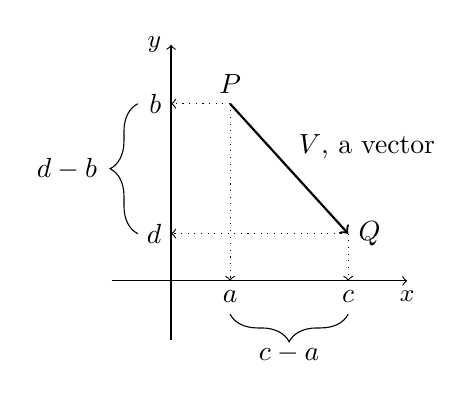
\begin{tikzpicture}[scale=1.5]
\draw[->] (-.5,0) -- (2,0) node[below] {\small $x$};
\draw[->] (0,-.5) -- (0,2) node[left] {\small $y$};
\draw[->,thick] (1/2,3/2) node[above] {$P$} -- (3/2,2/5) node[right] {$Q$};
\node [above right] at (1,19/20) {$V$, a vector};
\draw[dotted,->] (1/2,3/2) -- (1/2,0) node[below] {$a$};
\draw[dotted,->] (1/2,3/2) -- (0,3/2) node[left] {$b$};
\draw[dotted,->] (3/2,2/5) -- (3/2,0) node[below] {$c$};
\draw[dotted,->] (3/2,2/5) -- (0,2/5) node[left] {$d$};
\draw[decorate,decoration={brace,amplitude=10pt},xshift=-8pt,yshift=0pt] (0,2/5) -- (0,3/2) node[midway,xshift=-.9cm] {$d-b$};
\draw[decorate,decoration={brace,mirror,amplitude=10pt},xshift=0pt,yshift=-8pt] (1/2,0) -- (3/2,0) node[midway,yshift=-.5cm] {$c-a$};
\end{tikzpicture}
\caption{Coordinates for a physicist's vector $V$.}
\end{figure}


Then the coordinates of $V$ are taken to be the $(c-a, d-b)$, which we interpret how much $V$ acts in the directions parallel to the $x$-axis and the $y$-axis, respectively.

%Notes: (1) subtraction???? $Q-P$?  (2) ambiguity over location...

Note that these coordinates have a hint of algebraic manipulation in them. 
Those subtractions line up almost like we could write $V =(c-a,d-b) = (c,d)-(a,b) = Q-P$. 
But that would mean that we are subtracting points and creating a vector, which is weird.
We will return to this idea soon.

For now, let's focus on a bit of ambiguity in the physicist's idea of a vector. 
Where should that vector be?
That is, given the coordinates of a vector in the plane, it is not clear where to draw it!
I can slide a vector around the plane, and as long as I keep it parallel to the original, the coordinates won't change. 
So, unlike with the coordinates of a point, the coordinates of a vector do not uniquely specify the vector.

The mathematician's special fix is this: we simply declare all our vectors to have their initial points, their tails, at the origin $O$, of our coordinate system.
That curtails some of the (admittedly useful) freedom in the physics notion, but it also lets us be more clear.

\begin{figure}[h]
\centering
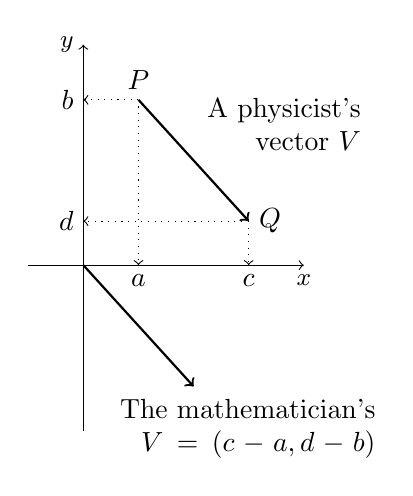
\begin{tikzpicture}[scale=1.4]
\draw[->] (-.5,0) -- (2,0) node[below] {\small $x$};
\draw[->] (0,-1.5) -- (0,2) node[left] {\small $y$};
\draw[->,thick] (1/2,3/2) node[above] {$P$} -- (3/2,2/5) node[right] {$Q$};
\node [text width=2cm,align=right,above right] at (1,19/20) {A physicist's vector $V$};
\draw[dotted,->] (1/2,3/2) -- (1/2,0) node[below] {$a$};
\draw[dotted,->] (1/2,3/2) -- (0,3/2) node[left] {$b$};
\draw[dotted,->] (3/2,2/5) -- (3/2,0) node[below] {$c$};
\draw[dotted,->] (3/2,2/5) -- (0,2/5) node[left] {$d$};
\draw[->,thick] (0,0) -- (1,-11/10);
\node [text width=3.5cm,align=right,below] at (7/5,-9/8) {The mathematician's \\$V = (c-a,d-b)$};
\end{tikzpicture}
\caption{The physicist's vector vs. the mathematician's vector.}
\end{figure}

But it pays to keep in mind that the physicists conception of the vector $V = (c-a,d-b)$ could be one of many different arrows, while the mathematician's vector $V$ is the arrow from the point $O = (0,0)$ to the point $(c-a, d-b)$.

Now we have circled back around to a muddle. If a mathematician's vector is always based at $O$, we only need to specify where the head of the vector is\dots which is just a point. So, how is a vector supposed to be different from a point, again? 

This confusion of three different, shifting, partially-overlapping interpretations causes some trouble to the new learner. Professionals tend to pass back and forth between these and use them flexibly to get results. Once you have gotten used to the ideas, you will, too. You should watch out for these instances where the words point and vector get interchanged. If they cause you trouble, remember that we have three different things, which are closely related.

For now, the simplest way to handle things is like this:
\begin{itemize}
\item A point is a location in the plane, and represented by coordinates in the form of an ordered pair of numbers $(a,b)$.
\item Ignore the physicist's version of the word vector as much as possible.
\item A vector is an arrow based at the origin, which can be specified by the coordinates of its head. To keep this separate from the idea of a point, we will write it differently, with the numbers stacked vertically like this: $\left(\begin{smallmatrix} a \\ b \end{smallmatrix}\right)$.
\end{itemize}
With this in mind, we make our first official definition.

\begin{definition} A $2$-vector is a vertical stack of $2$ real numbers, like so:
\[
v = \begin{pmatrix} a \\ b \end{pmatrix}.
\]
The collection of all such $2$-vectors is called \emph{the plane}, and written with this notation: $\R^2$.
\end{definition}

The notation $\R^2$ is often read ``arr-two,'' and many people use that language interchangeably with ``the plane.''


\section*{Lines as Parametric Objects}

\begin{compactitem}
\item vector algebra in R2
\item lines in R2 as parametric objects: through the origin, and not
\item sketching lines in R2
\end{compactitem}

\section*{Lengths and Angles in the plane}
\begin{compactitem}
\item lengths, angles, and the dot product in R2
\item normal vector to a line in R2
\item duality
\end{compactitem}


\begin{compactitem}
\item points vs physics vectors vs math vectors
\item the idea of R2
\item sketching points and vectors in the plane
\end{compactitem}


\section*{Lines and Equations}
\begin{compactitem}
\item equation of a line, three methods: elimination, from two pts via similar triangles, from geometry of dot product
\item families of parallel lines
\item sketching a line from an equation
\end{compactitem}

\section*{Conclusion: The Big Theorem}


\end{document}